% This is LLNCS.DEM the demonstration file of
% the LaTeX macro package from Springer-Verlag
% for Lecture Notes in Computer Science,
% version 2.4 for LaTeX2e as of 16. April 2010
%
\documentclass{llncs}
%
\usepackage{makeidx}  % allows for indexgeneration
%
\usepackage{graphicx}

\usepackage{mathtools}
\DeclarePairedDelimiter{\norm}{\lVert}{\rVert}

\setcounter{secnumdepth}{4} % seting level of numbering (default for "report" is 3).

% define a newline after subsubsection like subsection
\makeatletter
\renewcommand\subsubsection{\@startsection{subsubsection}{3}{\z@}%
	{-18\p@ \@plus -4\p@ \@minus -4\p@}%
	{4\p@ \@plus 2\p@ \@minus 2\p@}%
	{\normalfont\normalsize\bfseries\boldmath
		\rightskip=\z@ \@plus 8em\pretolerance=10000 }}
\makeatother


\begin{document}
%
\frontmatter          % for the preliminaries
%
\pagestyle{headings}  % switches on printing of running heads


%

%
\mainmatter              % start of the contributions
%
\title{Yelp Recommendation System Based on Collaborative Filtering}
%
\titlerunning{Yelp Recommendation System Based on Collaborative Filterings}  % abbreviated title (for running head)
%                                     also used for the TOC unless
%                                     \toctitle is used
%
\author{Sainan He, Jiaoyang Fu, Yameng Li}
%
\authorrunning{Ivar Ekeland et al.} % abbreviated author list (for running head)
%
%%%% list of authors for the TOC (use if author list has to be modified)
\tocauthor{Sainan He, Jiaoyang Fu, Yameng Li}
%
\institute{Electrical and Computer Engineering, University of Waterloo, Canada,\\
\email{{s66he, j45fu, y949li}@uwaterloo.cau}
}

\maketitle              % typeset the title of the contribution

\begin{abstract}
Based on Yelp Data Challenge dataset, we aim to develop a predictive personalized recommendation system on user’s review star rating for restaurants, applying collaborative filtering algorithms. In particular, we implement and compare the performances of four algorithms including baseline, User-based and Item-based collaborative filtering and Singular Vaule Deccomposition (SVD). We evaluate our results by comparing our predicted rating to the actual rating using Root Mean Squared Error(RMSE) and Mean Absolute Error(MAE) metrics.

\keywords{Recommendation System, Collaborative filtering, Singular Vaule Deccomposition (SVD), Yelp Data Challenge}
\end{abstract}

\section{Introduction}
With rapid development of advanced technology, people nowadays can achieve the things that they desired faster and more effectively than ever. While, at the same time, the requirements for accurate, personalized and convenient services are increasing. Fortunately, Yelp contributes to providing reasonable recommendations of various businesses to users, e.g., restaurants.

Yelp collected review dataset which records how well each user rates for limited amount of restaurants. Based on these review history, it suggests favored restaurants to users. The problem is that Yelp seems to offer similar recommendations that are popular for various users. In fact, people may have diverse preferences to food. For instance, some users may prefer Asian food, while others may favor Mexican food. In fact, yelp did not consider these factors too much. Therefore, it seems still have some room to improve the recommendation system in the personalization aspect.

Collaborative filtering, a method making predictions based on a large dataset used by some recommendation system like Yelp, Amazon, and Netflix. It automatically predict about the interests of a user by collecting preference or tastes information from other users. Furthermore, there are numerous collarborative filtering methods, such as baseline, K- nearest neighbor, and matrix decomposition. This paper aims to compare how accurate each methods applying on Yelp Data Challenge through using Root metric Mean Squared Error(RMSE) and Mean Aboslute Error(MAE).

\section{Literature Review}
There are generaly three types of recommendation systems: content-based filtering, collaborative filtering and hybrid approaches. Content-based recommendation systems work with users’ profile and items’ characteristics. The feature used to bulding profiles are often a set of keywords. For example, a music recommendation system\cite{MJ} implemented with content-based filtering, each song is assigned an attribute manually. If a user’s profile shows interests in songs with particular atrtibutes, similar songs will be recommended to the user. The limitations of these systems is that it always recommends similar items to user that he has already purchased and it’s difficult to recommend items for new users. 

Collaborative filtering try to predict the utility of items for a particular user based on the items previously rated by other users with similar tastes and preferences. In\cite{Bruno} the author builds a recommendation system for a retail store using three kinds of collaborative filtering algorithms - memory based approach, matrix factorization and bigram matrix method. Collaborative filtering also has limitations that it is difficult to recommend items for new users, to recommend items which have not been rated before, and to recommend when rating information is insufficient. 

Hybrid approach combines multiple techniques to overcome the limitations of individual systems. A restaurant recommendation system for yelp user\cite{Sumedh} adopts hybrid approach by extracting collaborative and content-based features to identify customer and restaurant profiles. A hybrid cascade of K-nearest neighbor clustering, weighted bi-partite graph projection, and several other learning algorithms are proposed. 

\section{Data}
We collect our data from Yelp recommendation Kaggle competition\cite{yelp},This dataset contains 11,537 businesses, 8282 check-in sets, 43873 users, and 229907 reviews. We target “Restaurant” in the city of “Phoenix” as it is more reasonable to recommend restaurants for users in the same city.

\subsection{ Data Processing}
The original data file is in json format. We firstly parse the raw data of imformation from users, businesses and reviews, respectively and merge them into one dataframe. Then we extract the records with features of “Restaurants” and “Phoenix” for futher analysis. After this approach, we have 17145 users, 1454 business and 52749 reviews.

Because many users only review a few restaurants, our dataset yields a sparsity of 99.79\% which can be visualized from figure 1. To solve this problem, we create a smaller dataset which only consider  restaurants reviewed by more than 50 users.
%

\begin{figure}
	\begin{minipage}[t]{0.5\textwidth}
		\centering
		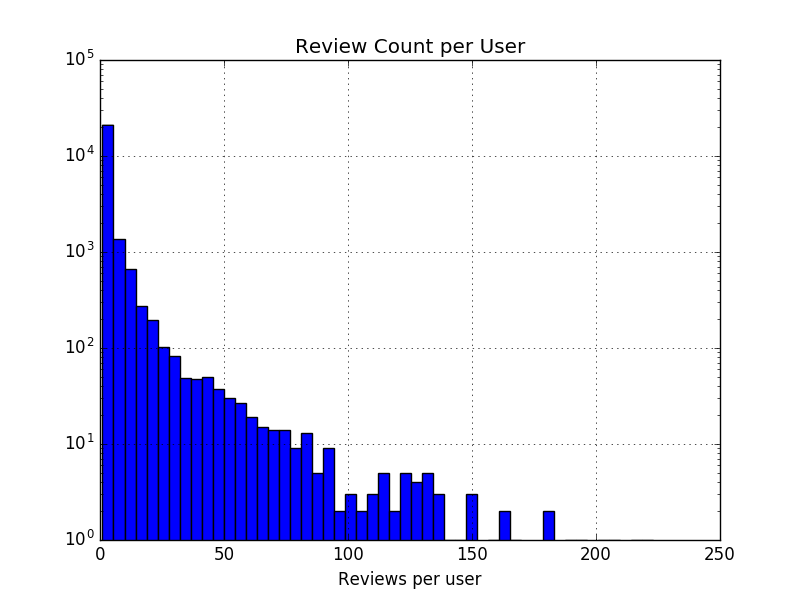
\includegraphics[width=2.2in]{fig1.png}
		\caption{User review count}
		\label{fig:side:a}
	\end{minipage}%
	\begin{minipage}[t]{0.5\textwidth}
		\centering
		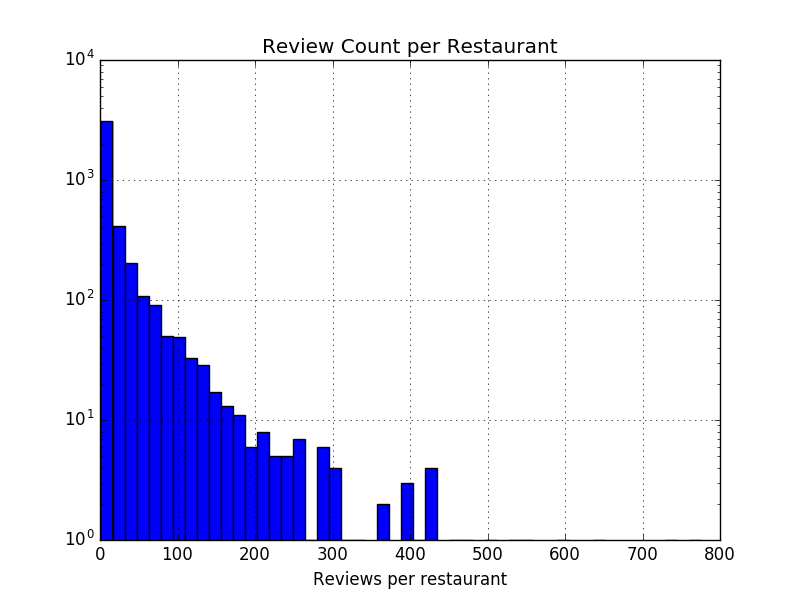
\includegraphics[width=2.2in]{fig2.png}
		\caption{Restaurants review count}
		\label{fig:side:b}
	\end{minipage}
\end{figure}

\subsection{Traing and Testing sets}
%
In order to evaluate the performance of our recommendation system, we divided our data into training and testing datasets. We extract a list of all restaurants each user has rated, take 80\% of this list as training set and 20\% as test set. 

\section{Methods}
\subsection{Baseline}
Our baseline model is similar to the model implemented by\cite{Yehuda} which is a mean predictor and accounts for the user and item effects. 
\begin{equation}
\ b_{ur} = \mu + b_u + b_r \ .
\end{equation}

Here $\mu$ is the mean rating of reviews of all business by all users. The parameter $b_{ur}$ indicates the difference between the average rating of user $u$ and $\mu$. The parameter bi indicates the difference between the average rating of business $i$ and $\mu$. This will normalize the widely noticed tendency of some user giving higher rating than others and some restaurants getting higher ratings than others.


\subsection{User-User Collaborative Filtering}
\textit{User-user collaborative filtering}, also know as \textit{k-NN collaborative},was the first of the automated CF methods. It find other users whose past rating behavior is similar to that of current user and
use their ratings on that item to predict what the current user will like. To predict Mary's preference for an item she has not rated, user-User CF looks for other users who have high agreement with Mary on the items they have both rated.These users’ ratings for the item in question are then weighted by their level of agreement with Mary’s ratings to predict Mary's rating on that item. 

\subsubsection{Computing Predictions}
To compute predictions or recommendations for a user u, user-user CF firstly needs to determine the number N of neighbors will be used to generate the result. Then computing the weighted average of the chosen neighboring users' rating i by using similarity as weights. The formula is given as below:

\begin{equation}
p_{u,i} ={\bar r_{u}}  + \frac
{\sum\nolimits_{u' \in N} s(u,u')(r_{u',i} - {\bar r_{u'}})} 
{\sum\nolimits_{u' \in N} |s(u,u')|}
\end{equation}

In order to eliminate the differences in users's use of the rating scale, subtracting the user's mean rating ${\bar r_{u'}}$ to compensate is necessary.   The parameter $p_{u,i}$ is predicated rating on item i for user $u$.  ${\bar r_{u'}}$ is average rating on all items rated by user $u$.The parameter $r_{u',i}$ indicates the rating of user $u'$ on item i.$s(u,u')$ is similarity between user u and $u'$. N is the number of neighbors chosen for user $u$.  



\subsubsection{Computing User Similarity}
An critical parameter used to calculate predications is similarity function.Among many proposed similarity functions we only choose Cosine Similarity to give a detailed introduction. 

In Cosine Similarity model, users are represented as $|\textit{I}|$-demensional vectors of rating on $|\textit{I}|$ items.Similarity is measured by the cosine distance between two rating vectors. The formula is given below indicating how to calculate the Cosine Similarity between user $u$ and $v$. 
\begin{equation}
s(u,v) = \frac{r_{u}\cdot r_{v}}{\norm {r_{u}}_{2} \norm {r_{v}}_{2}}=\frac{\sum\nolimits_{i} r_{u,i}r_{v,i}}{\sqrt{\sum\nolimits_{i} {r^{2}_{u,i}}} \sqrt{\sum\nolimits_{i} {r^{2}_{v,i}}}} 
\end{equation}

Unknown ratings are considered to be 0. $r_{u}$ is rating vector of user $u$. $\norm {r_{u}}_{2}$ is the Euclidean norm of rating vector $r_{u}$.

\subsection{Item-Item Collaborative Filtering}
\textit{Item-Item Collaborative Filtering} uses similarity between the rating patterns of items.If two items tend to have the same users like and dislike them,then they are similar and users are expected to have similar preferences for similar items.

\subsubsection{Computing Predictions}
To generate predictions or recommendations for user $u$ on item $i$, item-item CF firstly determine a set S of items most similar to $i$. Then computing the weighted average of the user's rating on item $j$ from set S. The formula is given as below:

\begin{equation}
p_{u,i} =\frac
{\sum\nolimits_{j \in S} s(i,j)r_{u,j}} 
{\sum\nolimits_{j \in S} |s(i,j)|}
\end{equation}

The parameter $p_{u,i}$ is predicated rating on item i for user $u$. $S$ is a set of items most similar to item $i$. $s(i,j)$ is the similarity between item $i$ and $j$. $r_{u,j}$ is the rating of user $u$ on item $i$.
\subsubsection{Computing Item Similarity}
As in user-user collaborative filtering, a variety of methods can be used for computing item similarity. In this section, we focus on Cosine Similarity, the most popular similarity metric, as it is simple, fast, and produces good predictive accuracy. 

\begin{equation}
s(i,j) = \frac{r_{i}\cdot r_{j}}{\norm {r_{i}}_{2} \norm {r_{j}}_{2}}
\end{equation}

Unknown ratings are considered to be 0. $r_{i}$ is rating vector of item $i$. $\norm {r_{i}}_{2}$ is the Euclidean norm of rating vector $r_{i}$.


\subsection{Singular Value Decomposition}

\section{Experiments and Results}
%
\subsection{Evaluation Metrics}
Our goal is to predict the rating a user would give to a restaurant. We predict the rating that user has not rated in the training dataset, but the true rating is stored in the test dataset. We use the root-mean-square error and mean-absolute error for evaluation.
\begin{equation}
\ RMSE = \sqrt{\frac{\sum{\left(r'_{u,i} - r_{u,i}\right)}^2}{N}}
\end{equation}
\begin{equation}
\ MAE = \sqrt{\frac{\sum{\left|r'_{u,i} - r_{u,i}\right|}}{N}}
\end{equation}

Here $r_{u,i}$ is the predicted rating from user $u$ on item $i$ and $r'_{u,i}$ is the true rating; $N$ is the size of test dataset. 

\section{Results}
The performance of our baseline predictor is $RMSE = $, $MAE= $.


\end{document}
